\documentclass[nonacm,screen]{acmart}
\pdfoutput=1
\usepackage{graphicx}
\usepackage{pifont}

\newcommand\V[1]{\textsc{\MakeLowercase{#1}}}

\AtBeginDocument{\libertineOsF}

\begin{document}

\title{Putting the Count Back Into Accountability}
\subtitle{An Audit of Social Media Transparency Disclosures,
    Focusing on Sexual Exploitation of Minors}

\author{Robert Grimm}
\orcid{0000-0002-8300-2153}
\affiliation{%
    \institution{Independent Investigator}
    \city{Brooklyn}
    \state{New York}
    \country{United States}
}
\email{rgrimm@alum.mit.edu}

\begin{abstract}
This paper explores a lightweight, quantitative audit methodology for
transparency disclosures called \emph{scrappy audits}. It amounts to little more
than treating redundant and repeated disclosures as opportunities for validating
quantities. The paper applies two concrete audits to social media disclosures
about content moderation. The first compares legally mandated reports about the
sexual exploitation of minors as disclosed by social media and the national
clearinghouse receiving them. The second compares historical quantities included
in platforms' \V{CSV} files across two subsequent disclosures of the data.
Despite their simplicity, these scrappy audits are nonetheless effective. Out of
16 surveyed social media platforms, 11 make transparency disclosures about
content moderation and 8 meet the prerequisites of one audit. Yet only
4~platforms pass their audits. The paper continues probing the limits of
transparency data by presenting a data-driven overview of the online sexual
exploitation of minors. Accordingly, the analysis is particularly careful to
identify threats to validity as well as potentially helpful, but unavailable
statistics. Likewise, it identifies major shortcomings of widely used
technologies for the automated detection of images and videos depicting sexual
abuse of minors. Overall, the data shows an alarming growth in such material
over the last decade. However, there also are strong indicators that current
statistics, which treat all such material the same, are large and unhelpful
overcounts. Notably, many technical violations of the law, e.g., teenagers
sexting, are not necessarily grounded in actual harm to minors but still
reported as such.
\end{abstract}

\begin{CCSXML}
<ccs2012>
<concept>
<concept_id>10003456.10003462</concept_id>
<concept_desc>Social and professional topics~Computing / technology policy</concept_desc>
<concept_significance>500</concept_significance>
</concept>
<concept>
<concept_id>10002951.10003227.10003233.10010519</concept_id>
<concept_desc>Information systems~Social networking sites</concept_desc>
<concept_significance>500</concept_significance>
</concept>
</ccs2012>
\end{CCSXML}

\ccsdesc[500]{Social and professional topics~Computing / technology policy}
\ccsdesc[500]{Information systems~Social networking sites}

\keywords{social media, content moderation, transparency reporting, audit, minor
safety, sexual exploitation of minors, child sexual exploitation, child sexual
abuse material, CSAM, CyberTipline, National Center for Missing and Exploited
Children, NCMEC, teenage sexting}

\maketitle


% ======================================================================================

\section{Introduction}
\label{sec:introduction}

The work described in this paper started with the question: Can an interested
individual, without institutional backing and without privileged access to
social media platforms, make an objective determination about the accuracy of
transparency disclosures on content moderation? While the question's
preconditions reflect my own status as independent researcher, the question has
broader relevance, applying to people interested in performing open source
intelligence or strengthening civil society just as well. By exploring the
limits of individual agency, the question may have broader relevance still. But
the posture of underdog fighting corporate behemoths would also be misleading,
since I worked as software engineer for Facebook from 2018 to 2019. However, I
did \emph{not} work on content moderation and I do \emph{not} retain any
financial interest in the firm.

In looking for such \emph{scrappy audits}, I soon realized that redundant and
repeated disclosures of the same metric, especially when originating from
different organizations, provide just the desired opportunities for validating
disclosed statistics because every divergence is a true positive error. That
immediately led to the first audit. Compare so-called CyberTipline report counts
disclosed by social media with those by the national clearinghouse receiving the
reports, the National Center for Missing and Exploited Children or \V{NCMEC}.

The second audit was the result of a series of fortunate events, even if they
didn't look it at first. After refactoring my code for analyzing Meta's \V{CSV}
files, I carefully compared outputs to ensure that the new version still worked
as expected. When numbers didn't match, I first reviewed my code and, finding
nothing wrong, next checked the programs' inputs. After noticing that I was
using the \V{CSV} file for \V{Q3}~2022 instead of \V{Q2}~2022, I compared all
quantities between the two files besides values newly added in \V{Q3} and
discovered that 113 out of 2,633 or 4.3\% of quantities differed, 77 of them
dating back to \V{Q4}~2020. I had found the cause for the divergent
outputs---and the second audit for this paper!

Neither of the two audits requires more than a computer capable of running basic
data analysis tasks---datasets easily fit into memory and the most ``complex''
math in this paper is a least-squares-fit over a log function---as well as as
some time and attention to detail while extracting statistics from \V{HTML} and
\V{PDF} files to make them machine-readable. In case of disclosures about the
sexual exploitation of minors, you wouldn't even need the latter, since I
already did the work and publicly released all code and
data.\footnote{\label{fn:intransparent}\url{https://github.com/apparebit/intransparent}}
In short, the two audits definitely qualify as scrappy and enable interested
individuals to do their own research---without all the downsides so often
associated with just that phrase. Yet despite the methodology's simplicity, this
type of investigation still is novel. Besides a parallel investigation comparing
transparency disclosures under the \V{EU}'s Digital Services Act and the
corresponding statements of reasons database
statistics~\cite{TrujilloFagniea2024}, I am not aware of similar studies.

The audits also are effective. Out of 16~surveyed social media platforms, 11
make transparency disclosures about content moderation and 8 meet the
prerequisites of one audit each. Yet only 4~platforms pass their audits. That's
pretty remarkable since all but one of the surveyed platforms have been
operational for at least a decade and engage in surveillance
capitalism~\cite{Zuboff2019}. In other words, they should excel at the data
collection and analysis tasks necessary for transparency disclosures. Yet the
failures are substantial. Notably, in the case of Meta's \V{CSV} files,
differences for the previous quarter might, in theory, stem from corrections
applied after the quarterly reporting deadline. But \V{IRL}, seven successive
pairs of quarters have substantial differences across all kinds of metrics
dating back up to two years. Hence Facebook and Instagram clearly fail that
audit.

This paper makes three contributions. First, previous audits of social media
tranparency disclosures focus either on overall scope and semantics of such
disclosures including metrics or compare measured user experience with
platforms' claims~\cite{AccessNow2021,CrockerGebhartea2019,Francoisdouek2021,
StoughtonRosenzweig2022,WagnerRozgonyiea2020}. That also seems to be the case
for the two audits Meta commissioned~\cite{BradfordGriselea2019,Meta2022,
Plumb2019,Sarang2022}. As far as I know, the focus on auditing the data itself
is unique to this work. It also is complementary to previous work and thereby
contributes towards a more holistic understanding of social media transparency
disclosures. Second, a critical preparatory aspect of the work was the curation
of transparency data in machine-readable form and the development of the
analysis code. Both have been released as open source.\footnote{See
footnote~\ref{fn:intransparent}} Third, right-wing activists have been
instrumentalizing the sexual exploitation of minors as a political
cudgel~\cite{BuntainBarlowea2022,Feffer2021,Gilbert2023, Romano2022}. To counter
their manipulative appeals to strong emotions, I provide an evidence-based
overview of what transparency disclosures tell us about the online sexual
exploitation of minors, with a focus on social media from 2019 to 2022. Along
the way, I am careful to identify threats to validity and topics missing
entirely from the data, while also validating previously published work.


% ======================================================================================

\section{Background and Related Work}
\label{sec:background}

\subsection{US Law}

Chapter 110 of 18 \V{US} Code~\cite{Chapter110Code18US}, the United States'
primary criminal code, concerns the ``sexual exploitation and other abuse of
children'' (the chapter's title) and prohibits grooming children (\S2251),
selling or buying children (\V{\S2251A}), the production, distribution, and
possession of sexually explicit imagery involving minors (\S2252) including
child pornography (\V{\S2252A}) even in other countries (\S2260), and tricking
minors into accessing harmful materials with misleading domain names
(\V{\S2252B}) or page contents (\V{\S2252C}). As long as providers of electronic
services immediately report such activities and materials to \V{NCMEC}'s
CyberTipline (\V{\S2258A}), it explicitly limits their civil and criminal
liability (\V{\S2258B}), which otherwise includes criminal (\S2253) and civil
forfeiture (\S2254) as well as mandatory restitution (\S2259) in addition to
long prison sentences, e.g., 5--20 years for the first violation of \V{\S2252A}
and 15--40 years for subsequent violations.

Chapter 110 also establishes \V{NCMEC} as a clearinghouse for information about
the sexual exploitation of minors. It requires \V{NCMEC} to forward CyberTipline
reports to suitable law enforcement agencies (domestic and foreign alike,
\V{\S2258A}). It also authorizes \V{NCMEC} to collect hashes and other
identifying information for reported imagery and share that information with
service providers (\V{\S2258C}). That puts \V{NCMEC} into a rather unique
position. It works closely with both industry and law enforcement. Similarly,
while its role is established through the United States criminal code, the
organization itself is a \emph{private} non-profit corporation. The
Congressional Research Service has documented the relevant background and
history~\cite{FernandesAlcantaraHanson2021}. As far as CyberTipline reports are
concerned, the documentation for the bulk \V{API} used by electronic service
providers is public~\cite{NCMEC2024}. Furthermore, individual reports have been
disclosed in the course of legal proceedings, of course without any
attachments~\cite{NationalCenterForMissingAndExploitedChildren2017,
NationalCenterForMissingAndExploitedChildren2017a}.


\subsection{Transparency Reporting and Audits}

Transparency disclosures about content moderation---and hence the need for
auditing them---are a relatively recent phenomenon emerging from the confluence
of three trends. First, news of Russia's covert disinformation campaign during
the 2016 \V{US} presidential election~\cite{Francoisdouek2021}, the spread of
medical and public-health misinformation during the \V{COVID-19}
pandemic~\cite{ChoLiea2023,FoleyGurakar2022,GreenhalghOzbilginea2022},
misinformation during the 2020 \V{US} presidential election and the subsequent
attempted coup, as well as the trove of Meta's internal documents released by
Frances Haugen~\cite{CameronWodinskyea2023,ElliottChristopherea2021} kept
reminding the public of social media's corrosive influence and increasing
demands for better accountability about content
moderation~\cite{HaimsonDelmonacoea2021,KozyrevaHerzogea2023}. Increasing use of
algorithmic decision systems, notably at the beginning of the pandemic, only
intensified the pressure on social media~\cite{ScottKayali2020}.

Second, while researchers used to have broad \V{API}-based access to platform
data including individual posts, social media firms severely restricted or
phased out bulk access in the aftermath of the scandal caused by Cambridge
Analytica siphoning huge amounts of user data from
Facebook~\cite{Bruns2019,Puschmann2019,WalkerMerceaea2019}. When \V{AI} startups
leveraged, amongst many other sources, Reddit's and Twitter's content for
training large language models, the affected platforms responded by instituting
hefty charges for access to remaining \V{API}s, making them unaffordable even
for most commercial applications~\cite{Isaac2023}.

Third, internet platforms originally started making transparency reports to hold
governments accountable after Edward Snowden's leak of secret government
documents revealed extensive communications surveillance by the United States'
clandestine services in cooperation with their Australian, British, and Canadian
counterparts. After Google released its ``Government Requests Tool'' in 2010,
other internet platforms started making similar
disclosures~\cite{TrustSafetyProfessionalAssociation2022}. By now, all but three
of the 16~platforms surveyed for this article regularly disclose government
requests for user information as well as content removal.

Etsy was the first internet platform to release a transparency report about
content moderation in 2015. Two years later, Germany's NetzDG law required them
for actions performed in response to its dedicated flagging
mechanism~\cite{TrustSafetyProfessionalAssociation2022}. YouTube was the first
social media platform to release a transparency report about content moderation
in 2018, followed by Facebook and Twitter that same year, Reddit in 2019, and
Pinterest, Snap, as well as TikTok in 2021~\cite{Binder2018,York2018}. While
some civil society organizations have been content at simply tracking firms that
make any transparency disclosures~\cite{AccessNow2021,StoughtonRosenzweig2022},
the Santa Clara Principles, released in 2018 and revised in 2021, capture the
civil society consensus on best
practices~\cite{AccessNowACLUFoundationOfNorthernCaliforniaea2021}. At least
Reddit and Twitter acknowledged as much by paying lip service to the Santa Clara
Principles in their transparency disclosures~\cite{Reddit2022,Twitter2022}.
Alas, no social media platform comes even close to complying with them
\V{IRL}~\cite{UrmanMakhortykh2023}.

That is not surprising given that transparency disclosures about content
moderation, unlike earlier disclosures about government requests, always played
a more ambiguous role. While academics and civil society would like to treat
them as an accountability mechanism, social media also treat them as a means for
deflecting criticism. Hence Meta's and Twitter's disclosures prominently
highlight seemingly random metrics that make them look good. Meanwhile Reddit
can't commit to the metrics it discloses, changing some of them every reporting
period. Reddit also managed to bamboozle the Electronic Frontier Foundation into
believing that it provided notifications for all its content takedowns when it
simply doesn't~\cite{CrockerGebhartea2019,Hawkins2023}.

The obvious means for addressing the low quality and disparity of transparency
disclosures would seem to be legal mandates. However, so far, extreme
polarization and the resulting political gridlock in Washington, \V{DC} have
proven stronger. Judging by the Harvard Law Review debate about the straw man of
a non-existent ``standard picture'' for content
moderation~\cite{Douek2022,Kadri2022,Klonick2023,MinowMinow2023}, American legal
scholars are just as gridlocked.

Meanwhile the \V{EU} has been moving ahead with comprehensive regulation of the
technology industry, leading to the Brussels effect~\cite{Bradford2020}. For
purposes of this paper, the relevant law is the Digital Services Act or
\V{DSA}~\cite{EuropeanParliamentAndCouncil2022}. To achieve its goal of creating
``a safer digital space,'' the law places comprehensive obligations on platforms
with respect to identifying and managing systemic risks, flagging illegal
content, fairness and transparency of content moderation, assured compliance
with the act, and so on. At the same time, the \V{DSA} is designed to be
proportionate and differentiates by service functionality---from all
intermediary services to hosting services to online platforms---and service
size---from small to regular to very large---with small services generally
exempted and very large online platforms having the most obligations.
Additionally, requirements were gradually phased in between November 2022 and
February 2024.

Critically, the \V{DSA} mandates that online platforms including social media
notify users of content moderation decisions and provide a \emph{statement of
reason} or \V{SoR}. Furthermore, it requires that online platforms make at least
yearly transparency disclosures with aggregate information in machine-readable
form in addition to submitting those same statements of reasons ``without undue
delay'' to the \V{EU} Commission's database at
\url{https://transparency.dsa.ec.europa.eu}. Very large online platforms also
need to identify and mitigate systemic risks (arguably the \V{DSA}'s most
flexible and substantial instrument), provide accredited researchers with access
to their data, and submit to external audits for their overall compliance with
the \V{DSA}.

The inclusion of audits in the \V{DSA}'s obligations prompted civil society
organizations to explore audits and their
methodologies~\cite{ActionCoalitionOnMeaningfulTransparency2023,AdaLovelaceInstitute2021,
BhatiaAllen2023,CostanzaChockRajiea2022,MessmerDegeling2023}. Alas, the \V{EU}
Commisssion sidestepped questions about the details of audit methodology in its
final rules by largely focusing on the elaboration of platform and audit
risks~\cite{EuropeanCommission2023}. Interestingly, a first examination of the
statements of reasons database shows distinct degrees of compliance and
significant divergence from initial \V{DSA} transparency disclosures, thus
pointing to more opportunities for scrappy audits~\cite{TrujilloFagniea2024}.

Alas, Meta's two voluntary audits of its transparency disclosures nicely
illustrate how scope determines effectiveness. The first audit questioned a
panel of academic experts on suitable metrics and resulted in an informative,
well-reasoned document~\cite{BradfordGriselea2019,Plumb2019}. The second audit
asked certified public accountants to review ``Meta's management assertion'' of
the transparency disclosures for \V{Q4}~2021~\cite{Meta2022,Sarang2022}. While
Meta's blog post suggests a comprehensive and in-depth review, the actual
management assertion and public accountants' letter do not include any concrete
``controls'' that were, in fact, investigated. Both documents are also dated on
the same day. That raises significant doubts about the extent of the audit.
Hence, it isn't particularly surprising that the audit missed all short-comings
identified in this paper.


\subsection{Terminology}
\label{sec:terminology}

While the title of Chapter~110, 18~\V{US} Code references ``children,'' section
paragraphs are expressed in terms of \emph{minor}, i.e., per \S2256 ``any person
under the age of eighteen years.'' The same section also defines \emph{child
pornography} in terms of minor. In contrast, \V{NCMEC} uses \emph{child sexual
abuse material} or \V{CSAM}. Others use \emph{child sexual exploitation and
abuse imagery} or \V{CSEAI}. In my mind, the two terms are synonymous and either
seems preferrable over child pornography because they more clearly delineate
illegal imagery featuring minors from legal adult pornography. In contrast,
\emph{child sexual exploitation} or \V{CSE} is more general and covers, for
example, grooming and trafficking as well.

Throughout this paper, I generally use minor instead of child---even if
\V{ECPAT}'s terminology guidelines make a rather convoluted argument for the
opposite~\cite{GreijerDoek2016}. Not only is minor the legally accurate term,
but informal usage of child tends to imply prepubescence and child sexual
anything increasingly has inflammatory, politicized impact. Nonetheless, when
referring to imagery depicting the sexual abuse of minors, I follow \V{NCMEC}'s
precendent and use the acronym \V{CSAM}. Furthermore, when discussing the
transparency disclosures of a particular platform, I use the platform's
terminology, including the acronyms defined in the previous paragraph. Finally,
since CyberTipline reports are called just that, reports, I use the term
\emph{transparency disclosure} to avoid confusion between the two types of
reports.

During my research, I encountered a number of news articles referring to the
National Center on Sexual Exploitation (\V{NCOSE}) as if it was \V{NCMEC}.
Previously known as Morality in Media, that organization is a right-wing
advocacy group with a deeply homophobic and sexphobic
history~\cite{WikipediaNCOSE}. Since its re-branding in 2015, it has softened
some of its more extreme positions. It even tried to ingratiate itself with the
\V{LGBTQ+} community~\cite{Hawkins2023a}. Alas, disavowing one of its worst
smears does not make a sincere apology. Furthermore, it doesn't help that the
same blog post insists that \V{NCOSE}'s sexphobic opposition to all pornography
and sexwork is supportive of the community.


% ======================================================================================

\section{Scrappy Audits of Social Media Transparency Reports}
\label{sec:audits}

\begin{table}
\centering\libertineLF
\caption{Social media platforms and their transparency disclosures}
\label{tab:platform-overview}
\setlength{\tabcolsep}{0}
\begin{tabular}{@{\;}l@{\:\:}l@{\:\:}l@{\:\:}l@{\;}l@{\:\:}l@{\:\:}c@{\;}}
\textbf{Platform} & \textbf{Terminology} & \textbf{Metrics} &
\multicolumn{2}{l}{\textbf{Coverage}} &
\multicolumn{2}{l}{\textbf{Format} \hfill \textbf{Audit}\ \ } \\ \hline

\href{https://transparency.fb.com/reports/community-standards-enforcement/}{Facebook}
& \V{CSE} & rounded piece counts & Q & Q3~2018-- & one \V{HTML} page, \V{CSV} & \ding{56} \\

\href{https://transparencyreport.google.com/child-sexual-abuse-material/reporting}{Google}
& \V{CSAM} & piece \& report counts & H & H1~2020-- & one \V{HTML} page & \ding{52} \\

\href{https://transparency.fb.com/reports/community-standards-enforcement/}{Instagram}
& \V{CSE} & rounded piece counts & Q & Q2~2019-- & one \V{HTML} page, \V{CSV} & \ding{56} \\

\href{https://about.linkedin.com/transparency/community-report}{LinkedIn}
& child exploitation & piece counts & H & H1~2019-- & one \V{HTML} page & $\cdots$ \\

\href{https://www.microsoft.com/en-us/corporate-responsibility/digital-safety-content-report}{Microsoft}
& \V{CSEAI} & piece counts & H & H1~2020-- & Excel file/period & $\cdots$ \\

\href{https://policy.pinterest.com/en/transparency-report}{Pinterest}
& \V{CSE}, \V{CSAM} & piece \& report counts & Q/H & H1~2020-- & two \V{HTML} pages  & \ding{56} \\

Quora & $\cdots$ & $\cdots$ & $\cdots$ & $\cdots$ & $\cdots$ & $\cdots$ \\

\href{https://www.redditinc.com/policies/transparency}{Reddit}
& minor sexualization, \V{CSAM} & piece \& report counts & H & 2021-- & \V{HTML} page/period & \ding{52} \\

\href{https://values.snap.com/privacy/transparency}{Snap}
& \V{CSEAI} & piece \& report counts & H & H2~2019-- & \V{HTML} page/period & \ding{52} \\

Telegram & $\cdots$ & $\cdots$ & $\cdots$ & $\cdots$ & $\cdots$ & $\cdots$ \\

\href{https://www.tiktok.com/transparency/en/community-guidelines-enforcement-2023-3/}{TikTok}
& sexual exploitation of minors & piece fractional share & Q & Q1~2022-- & \V{HTML} page/period, \V{CSV} & \ding{56} \\

\href{https://transparency.automattic.com}{Tumblr}
& $\cdots$ & $\cdots$ & $\cdots$ & $\cdots$ & $\cdots$ & $\cdots$  \\

\href{https://transparency.twitter.com/en/reports/rules-enforcement.html}{Twitter}
& \V{CSE} & unique piece counts & H & H2'18--H1'22 & one tabbed \V{HTML} page & $\cdots$  \\

WhatsApp & $\cdots$ & $\cdots$ & $\cdots$ & $\cdots$ & $\cdots$ & $\cdots$  \\

\href{https://transparency.automattic.com}{Wordpress}
& $\cdots$ & $\cdots$ & $\cdots$ & $\cdots$ & $\cdots$ & $\cdots$  \\

\href{https://transparencyreport.google.com/child-sexual-abuse-material/reporting}{YouTube}
& \V{CSAM} & piece \& report counts & H & H1~2020-- & one \V{HTML} page & \ding{52} \\ \hline

\href{https://www.missingkids.org/cybertiplinedata}{\V{NCMEC}}
& \V{CSAM} & report counts & Y & 2019-- & \V{PDF}/table & $\cdots$  \\
\end{tabular}
\end{table}

In selecting platforms for my scrappy audits, I started with Buffer's list of
the 20 most popular platforms in 2022~\cite{Lua2022}, dropped the five platforms
targeting China because they are unlikely to adhere to the same governance
standards, dropped Facebook Messenger because it is part of the already included
Facebook, replaced Microsoft Teams and Skype with Microsoft because the firm
does not offer more granular transparency disclosures, and added Tumblr because
it became a destination for users leaving Twitter as well as employees laid off
by the firm in the wake of Elon Musk's takeover~\cite{Patel2022}. Finally, to
cover all platforms owned by the same corporate parent, I added Google and
Wordpress. When compared to the \V{EU}'s list of very large online platforms and
search engines, my list does not include five e-commerce firms, three
adult-oriented platforms, and one not-for-profit. Like Microsoft, Google does
not make more granular transparency disclosures. Hence my list contains Google
only once, whereas the \V{EU} distinguishes between Search, Play, Maps, and
Shopping in addition to YouTube, which is included in both lists.

Table~\ref{tab:platform-overview} provides an overview of the selected platforms
and their transparency disclosures about the sexual exploitation of minors. In
addition to platform names, which link to the platform's transparency
disclosures where available, the table comprises the following columns:
\emph{Terminology} lists the terms used to identify violative content as
introduced in Section~\ref{sec:terminology}. \emph{Metrics} indicates disclosed
quantities, with \emph{pieces} referring to individual photos and videos and
\emph{reports} referring to CyberTipline reports. \emph{Coverage} lists the
granularity of disclosures and the covered calendar range, using Q for
quarterly, H for semiannually, and Y for yearly. Pinterest is designated Q/H
because its statistics are calculated per quarter but released only
semiannually. Reddit is designated H but lists a start year because the firm
started out making annual disclosures but then switched to semiannual ones in
2022. \emph{Format} indicates the format of disclosures, and \emph{Audit} shows
the platform's audit performance.

A quick glance at the table suffices for determining that five out of the 16
surveyed platforms make no transparency disclosures about the sexual
exploitation of minors. In fact, Telegram makes no transparency disclosures at
all, whereas Quora and WhatsApp have made only legally required, minimal privacy
disclosures. Meanwhile, Automattic does make regular disclosures for Tumblr and
Wordpress, but only covering government requests and intellectual property.

Only a little less obvious is the fact that only three out of 16 platforms make
disclosures in machine-readable format. Meta has been releasing \V{CSV} files
for Facebook and Instagram since \V{Q2}~2021. TikTok released Excel files from
\V{Q3}~2021 to \V{Q3}~2022 and has been releasing \V{CSV} files since. The
project's GitHub repository collects these \V{CSV} files. Since Meta simply
updates the file accessible through the same link every quarter, I have been
collecting quarterly snapshots since \V{Q2}~2022 and filled in previous releases
through the Internet
Archive.\footnote{\url{https://web.archive.org/web/20240000000000*/https://transparency.fb.com/sr/community-standards/}}
Microsoft's use of Excel files is curious because they only contain the data
points for the reporting period in a nicely formatted spreadsheet. Twitter's
transparency reports include a menu item to download \V{CSV} data but I never
could get that to work, even before Musk's takeover of the firm. The GitHub
repository also contains machine-readable versions of all other transparency
disclosures. I extracted them with ad-hoc scripts and advanced text editor
features where possible and otherwise fell back onto manual data entry.

Out of the sixteen platforms, Telegram is the only platform based outside of the
United States and hence not subject to 18 \V{US} Code \V{\S2258A}'s reporting
requirements. The other 15 platforms including TikTok are headquartered in the
\V{US} and hence \emph{are} subject. According to \V{NCMEC}'s transparency
disclosures, the 15 \V{US}-based platforms \emph{do} submit CyberTipline
reports. Alas, only five platforms belonging to four corporations disclose the
number of reports filed, enabling a comparison with \V{NCMEC}'s disclosures.
They are Google, Pinterest, Reddit, Snap, and YouTube. An additional three
platforms belonging to two corporations disclose their transparency data in
machine-readable form, enabling a comparison with previous disclosures. They are
Facebook, Instagram, and TikTok. The rest of this section discusses the detailed
audit findings; it is organized by platform but combines those owned by the same
corporation. I start with \V{NCMEC}.


\subsection{The National Center for Missing and Exploited Children}

In 2020, \V{NCMEC} started making transparency disclosures by releasing two
multipage \V{PDF} documents with a table each listing CyberTipline reports by
electronic service provider (\V{ESP})~\cite{NcmecByPlatform2019,
NcmecByPlatform2020,NcmecByPlatform2021,NcmecByPlatform2022} and country of the
suspected user~\cite{NcmecByCountry2019,NcmecByCountry2020,NcmecByCountry2021,
NcmecByCountry2020}. In 2022, the organization added a third \V{PDF} document
with a table listing notifications sent to
\V{ESP}s~\cite{NcmecNotifications2021,NcmecNotifications2022}. It also began
releasing an actual, written
report~\cite{NcmecCyberTipline2021,NcmecCyberTipline2022}. While the latter did
contain some of the same material, \V{NCMEC} provided a more complete and
meaningful accounting of its work only in 2023, when it released its report to
the Department of Justice's Office of Juvenile Justice and Delinquency
Prevention~\cite{NCMEC2023}. Section~\ref{sec:global-spread} makes extensive use
of the report and its data.

While making the data in \V{NCMEC}'s \V{PDF} files machine-readable again, I did
encounter data quality issues with the organization's breakdown of CyberTipline
reports by country. In particular, the data included two entries for the same
country, labelled ``French Guiana'' and ``Guiana, French;'' entries for the
Netherlands Antilles in addition to the three island states resulting from the
Antilles' split in 2010; Bouvet Island even though this subantarctic Norwegian
territory is an uninhabited nature preserve; and ``Europe,'' presumably meaning
the continent, in addition to pretty much all European countries. Taken
together, problematic countries account for less than 250 CyberTipline reports
per year from 2019 to 2022. Hence I dropped them.


\subsection{Meta: Facebook, Instagram, and WhatsApp}

\begin{figure}
\centering\libertineLF
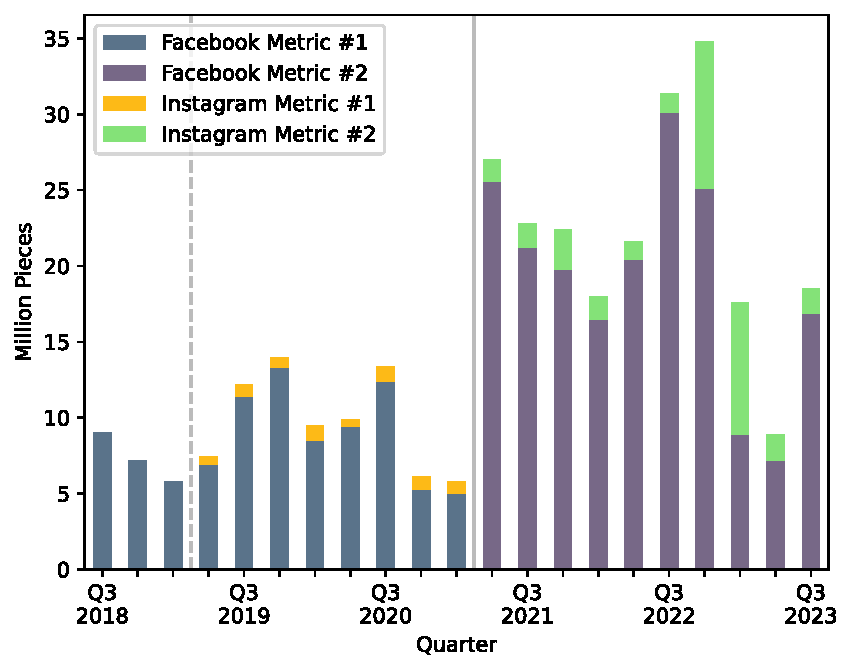
\includegraphics[
    scale=0.6,
    alt={Stacked bar graph illustrating combined quarterly counts for photos and
    videos depicting sexual exploitation of children on Facebook and Instagram.
    Underlying statistics changed substantially in \V{Q2}~2019 by adding
    Instagram and in \V{Q2}~2021 by updating the metric's definition.}
]{figure-meta-pieces}
\caption{Pieces maybe containing \V{CSE} on Facebook and Instagram (Meta)}
\Description{Stacked bar graph illustrating combined quarterly counts for photos
and videos depicting sexual exploitation of children on Facebook and Instagram.
Underlying statistics changed substantially in \V{Q2}~2019 by adding Instagram
and in \V{Q2}~2021 by updating the metric's definition.}
\label{fig:meta-pieces}
\end{figure}

Meta's transparency disclosures do not include CyberTipline reports but photos
and videos, or \emph{pieces}, that feature the sexual exploitation of children.
As indicated by the dashed vertical line in Figure~\ref{fig:meta-pieces}, Meta
originally collected that data for Facebook only and started to account for
Instagram as well with \V{Q2}~2019. As indicated by the solid vertical line and
different bar colors, Meta switched metrics from ``Child Nudity \& Sexual
Exploitation'' to ``Child Endangerment: Sexual Exploitation'' with \V{Q2}~2021.
While the names suggest that the former includes the latter metric, the jump in
piece counts that quarter suggests otherwise.

By searching for ``Meta Community Standards Enforcement Report \V{\V{Q2}}~2021''
with an external search engine, I eventually found a blog
post~\cite{Facebook2021a} linking a \V{PDF} document with the
explanation~\cite{Facebook2021}. The latter metric also includes ``Sexualization
of children'' and ``Inappropriate interactions with Children.'' While these
activities are related to minor safety as well, they don't seem obvious choices
for combination into a single metric. The fact that Meta did so anyways suggests
an ulterior motive, such as trying to impress readers by the sheer number of
successfully intercepted pieces. However, that is speculation on my part.

\begin{table}[h!]
\centering\libertineLF
\caption{CyberTipline reports for Meta (Meta and \V{NCMEC})}
\label{tab:meta-pieces-and-reports}
\begin{tabular}{lrrrr}
\textbf{Year} & \textbf{Pieces} & $\pi$ & \textbf{Reports} & \textbf{\% Total} \\ \hline
2019 & 39,368,400 & 2.48 & 15,884,511 & 94.3 \\
2020 & 38,890,800 & 1.92 & 20,307,216 & 94.7 \\
2021 & 78,012,400 & 2.90 & 26,885,302 & 92.2 \\
2022 & 105,800,000 & 3.89 & 27,190,665 & 85.5 \\
\end{tabular}
\end{table}

Table~\ref{tab:meta-pieces-and-reports} provides a little more context by
relating Meta's piece counts to CyberTipline report counts and then identifying
Meta's share of \emph{all} CyberTipline report counts (as disclosed by
\V{NCMEC}). In this table (and several subsequent ones), the $\pi$ stands for
\emph{product} and the column shows the multiplicative factor relating reports
to pieces. Remarkably, Meta detects and reports roughly nine times as many
incidents involving the sexual exploitation of minors \emph{as everyone else
combined}! Yet despite its industry-leading efforts, Meta still misses sexually
exploitative activities targeted at minors on both Facebook and Instagram, with
pedophiles having dedicated groups and \V{CSAM} producers advertising their
wares~\cite{HorwitzBlunt2023,HorwitzBlunt2023a}.

At the same time, there is evidence that piece counts severely overstate the
problem. To improve prevention, Meta developed a taxonomy for capturing the
intent behind shared \V{CSAM}~\cite{BuckleyAndrusea2021}. It also started
displaying automated warnings tailored according to intent~\cite{Davis2021}.
While the firm did not report on longer-term outcomes of those warnings, it did
report some striking statistics about intercepted \V{CSAM}. Notably, 90\% of
pieces reported to \V{NCMEC} during October and November 2020 had been reported
before or were visually similar to previously reported content, with six videos
accounting for more than half of the reported content. Further analysis of 150
accounts reported to \V{NCMEC} during July and August 2020 as well as January
2021 showed that 75\% of them didn't share \V{CSAM} with malicious intent but
``for other reasons, such as outrage or in poor humor (i.e. a child's genitals
being bitten by an animal).'' Unfortunately, Meta has not been disclosing any
further statistics, though the firm recently announced its plans to do
so~\cite{Meta2023}.

As already discussed in Section~\ref{sec:introduction}, Meta's disclosures for
Facebook and Instagram diverge for some fraction of historical quantities.
Between \V{Q3}~2021 and \V{Q4}~2022, an average of 102 or 4.1\% of such
quantities differ every quarter, affecting a wide range of metrics and going
back years. But in \V{Q1}~2023, the number of affected values dropped sharply,
to 18 or 0.6\% and the next two quarters see no such divergent quantities. These
counts may very well be undercounts because of Meta's practice of rounding
quantities. If I were to speculate, timing points to the \V{EU}'s Digital
Services Act, with Meta reigning in data fluctuations just before the \V{EU}
Commission designated Facebook and Instagram as very large online platforms on
April 25, 2023 (which started the four-month clock to come into
compliance)~\cite{EuropeanCommission2023a}. Still, the verdict is clear:
Facebook and Instagram fail the audit.

Meta does not make meaningful transparency disclosures for WhatsApp. However, as
\V{NCMEC}'s disclosures for 2021 and 2022 demonstrate, Meta does file
CyberTipline reports for WhatsApp: 1,372,696 in 2021 and 1,017,555 in 2022.


\subsection{Google and YouTube}

\begin{table}[h!]
\centering\libertineLF
\caption{CyberTipline reports for Google and YouTube (Google and \V{NCMEC})}
\label{tab:alphabet}
\begin{tabular}{l|rr|rrr}
\textbf{Year}
& \textbf{Pieces} & \textbf{$\pi$} & \textbf{Reports}
& \textbf{$\Delta\%$} & \textbf{NCMEC} \\ \hline
2019 & $\cdots$ & $\cdots$ & $\cdots$ & $\cdots$ & 449,283 \\
2020 & 4,437,853 & 8.10 & 547,875 & -0.2137 & 546,704 \\
2021 & 6,696,497 & 7.69 & 870,319 & 0.6278 & 875,783 \\
2022 & 13,402,885 & 6.16 & 2,174,319 & 0.0105 & 2,174,548 \\
\end{tabular}
\end{table}

\noindent{}Table~\ref{tab:alphabet} shows the combined number of pieces and
reports for Google and YouTube, tabulating Google's and \V{NCMEC}'s counts. The
difference is less than 0.7\% per year, which seems acceptable. Hence Google and
YouTube pass the audit.


\subsection{LinkedIn and Microsoft}

\noindent{}Even though Microsoft owns both LinkedIn and Skype, it treats
LinkedIn as a separate entity, with independent branding, logins, and
transparency reports, whereas Skype and Microsoft Teams are lumped in together
with the rest of Microsoft's services and hence also transparency disclosures.
Both Microsoft and LinkedIn report only pieces, not reports, and hence my audit
methodology does not apply.


\subsection{Pinterest}

\begin{table}[h!]
\centering\libertineLF
\caption{CyberTipline reports for Pinterest (Pinterest and \V{NCMEC})}
\label{tab:pinterest}
\begin{tabular}{l|rr|rrr}
\textbf{Year}
& \textbf{Pieces} & \textbf{$\pi$} & \textbf{Reports}
& \textbf{$\Delta\%$} & \textbf{NCMEC} \\ \hline
2019 & $\cdots$ & $\cdots$ & $\cdots$ & $\cdots$ & 7,360 \\
2020 & $\cdots$ & $\cdots$ & 3,432 & $\equiv$ & 3,432 \\
2021 & 1,608 & 0.599 & 2,684 & -14.94 & 2,283 \\
2022 & 37,136 & 1.127 & 32,964 & 4.08 & 34,310 \\
\end{tabular}
\end{table}

\noindent{}Table~\ref{tab:pinterest} shows the number of pieces and reports for
Pinterest, tabulating Pinterest's and \V{NCMEC}'s counts. The maximum difference
is almost 15\%, which seems too big an error. For divergent \V{CSV} data, the
responsible party is clear. For divergent CyberTipline report counts, it is
impossible to determine with certainty which side, Pinterest or \V{NCMEC} or
both, made tabulation errors. However, Pinterest is the more likely party, given
that \V{NCMEC}'s counts agree with those for the other audited platforms. While
both organizations would be well advised to validate disclosed quantities for
2021 and 2022, I attribute the failure to the likely culprit: Pinterest fails
the audit.


\subsection{Reddit}

\begin{table}[h!]
\centering\libertineLF
\caption{CyberTipline reports for Reddit (Reddit and \V{NCMEC})}
\label{tab:reddit}
\begin{tabular}{l|rr|rrr}
\textbf{Year}
& \textbf{Pieces} & \textbf{$\pi$} & \textbf{Reports}
& \textbf{$\Delta\%$} & \textbf{NCMEC} \\ \hline
2019 & $\cdots$ & $\cdots$ & 724 & $\equiv$ & 724 \\
2020 & $\cdots$ & $\cdots$ & 2,233 & $\equiv$ & 2,233 \\
2021 & 9,258 & 0.920 & 10,059 & $\equiv$ & 10,059 \\
2022 & 80,888 & 1.538 & 52,592 & $\equiv$ & 52,592 \\
\end{tabular}
\end{table}

\noindent{}Table~\ref{tab:reddit} shows the number of pieces and reports for
Reddit, tabulating both Reddit's and \V{NCMEC}'s counts. The counts aren't just
close, they are identical and Reddit passes the audit.

In the Electronic Frontier Foundation's latest audit in 2019, Reddit fared best,
receiving five out of five possible stars~\cite{CrockerGebhartea2019}. That
ranking is undeserved. First, Reddit changes some number of disclosed metrics
every report, which makes tracking changes impossible. Second, Reddit got one
star for providing meaningful notice upon taking down content. While it
committed to doing so when it touted its adherence to the Santa Clara Principles
in 2019~\cite{Reddit2022}, the firm doesn't do so in practice. Instead, Reddit
makes extensive use of shadow-banning, with content long deleted from Reddit
still appearing as visible to the users who posted it. Changing
``\texttt{reddit}'' to ``\texttt{reveddit}'' for any Reddit \V{URL} surfaces
such content for everyone~\cite{Hawkins2023}.


\subsection{Snap}

\begin{table}[h!]
\centering\libertineLF
\caption{CyberTipline reports for Snap (Snap and \V{NCMEC})}
\label{tab:snap}
\begin{tabular}{l|rr|rrr}
\textbf{Year}
& \textbf{Pieces} & \textbf{$\pi$} & \textbf{Reports}
& \textbf{$\Delta\%$} & \textbf{NCMEC} \\ \hline
2019 & $\cdots$ & $\cdots$ & $\cdots$ & $\cdots$ & 82,030 \\
2020 & $\cdots$ & $\cdots$ & $\cdots$ & $\cdots$ & 144,095 \\
2021 & $\cdots$ & $\cdots$ & $\cdots$ & $\cdots$ & 512,522 \\
2022 & 1,273,838 & 2.31 & 550,755 & 0.0601 & 551,086 \\
\end{tabular}
\end{table}

\noindent{}Table~\ref{tab:snap} shows the number of pieces and reports for Snap,
tabulating both Snap's and \V{NCMEC}'s counts. The difference is less than
0.07\%, which is acceptable. Snap passes the audit, albeit based on only one
pair of data points.


\subsection{Telegram}

Telegram does not make transparency disclosures. Furthermore, since it is
headquartered in Dubai, it does not need to report \V{CSAM} to \V{NCMEC}.
However, \V{NCMEC} reports that Telegram does respond, albeit slowly, to its
\V{CSAM} notifications. In 2021, Telegram received 229 notifications and took
8.0 days to act on average. In 2022, it received 73 notifications, taking 5.1
days to act on average. By comparison, the industry-wide response time in 2021
was 1.22 days on average.


\subsection{TikTok}

TikTok is one of only two surveyed companies to release transparency data in
machine-readable form. However, almost all data is of limited accuracy even in
the absence of data quality issues, since TikTok mostly discloses percentages
instead of counts. Furthermore, some of the data, including the \emph{sexual
exploitation of minors} subcategory of the \emph{minor safety} category, is
incomplete: TikTok reports the fractional share for the subcategory for human
moderation only, making it impossible to calculate the full count.

For the second quarter of 2023, TikTok updated its community guidelines,
including how it organizes violative categories. In its transparency report for
\V{Q2}~2023, the firm declared~\cite{TikTok2023}:
    \begin{quote}
    This report reflects our updated Community Guidelines, which took effect in
    April and provide our community with more transparency about our rules and
    how we enforce them. After consulting with more than 100 organizations
    globally, we overhauled how we organize our policies, simplified the
    language we use, and added granularity to help everyone, from creators to
    researchers, easily access the information they need. We’ve also refreshed
    various data visualizations to make them easier to read and understand,
    including for people with color vision deficiency.
    \end{quote}
However, in reality, category names and organization became more confusing and
less granular. The firm also continues to report fractional shares only.

To wit, before the update, the clearly named category \emph{minor safety}
included the sexual exploitation of minors, grooming behavior, physical and
psychological harm of minors, harmful activities by minors, as well as nudity
and sexual activity involving minors~\cite{TikTok2023a}. The five subcategories
are largely self-explanatory; though past transparency reports helpfully added
that the final subcategory largely comprises ``minors in minimal clothing'' and
``sexually explicit dancing.''

In contrast, consider the new category of \emph{safety \& civility}. Not only is
it obviously coarser, but its only seven subcategories also are clearly coarser.
Furthermore, their descriptions do not seem well
differentiated~\cite{TikTok2023}:
\begin{itemize}
    \item Harassment \& bullying: We do not allow language or behavior that
    harasses, humiliates, threatens, or doxxes anyone.
    \item Violent behaviors \& criminal activities: We do not allow violent
    threats, incitement to violence, or promotion of crimes against people,
    animals, or property.
    \item Violent \& hateful orgs \& individuals: We do not allow violent and
    hateful organizations or individuals, or the promotion or material support
    of them.
    \item Hate speech \& hateful behavior: We do not allow any hateful behavior,
    hate speech, or promotion of hateful ideologies.
    \item Human exploitation: We do not allow promoting or facilitating human
    exploitation, including trafficking and smuggling.
    \item Sexual exploitation \& gender-based violence: We do not allow showing
    or promoting physical, sexual or image-based abuse, sextortion, or sexual
    harassment
    \item Youth exploitation \& abuse: We do not allow any youth exploitation or
    abuse, including child sexual abuse material, pedophilia, or youth nudity.
\end{itemize}
To add insult to injury, subcategories and their explanations are only
accessible through tooltips when pointing to slices of an otherwise unmarked pie
chart. But even with the explanations, the distinctions between the first five
subcategories can be subtle and border on arbitrary. Worse, what used to be an
entire category with five subcategories, minor safety, now is just one
subcategory.

TikTok released Excel files from \V{Q3}~2021 through \V{Q3}~2022 and \V{CSV}
data thereafter. While data is already marred for the above stated reasons, we
can still determine quarter-over-quarter stability of historical disclosures.
Alas, the three comparisons between \V{Q4}~2022 and \V{Q3}~2023 (the latest
available) yield over 900 non-duplicated rows, each specifying a single
quantity, and that only after manually fixing column names to be consistent.
Spotchecks reveal the use of different names for what should be identical
categories and what appear to be unrounded floating point numbers. TikTok fails
the audit.


\subsection{Twitter}

Unlike other surveyed platforms, Twitter discloses counts of \emph{unique}
pieces. The idiosyncratic choice of metric seems designed to downplay the
problem and hence mislead readers. Related disclosures don't seem any better.
Consider 2021: Twitter disclosed 12,883 unique pieces that, per \V{NCMEC},
resulted in 86,666 CyberTipline reports. While that seems realistic, Twitter
also claims to have suspended 1,050,751 accounts for child sexual exploitation.
That's $12\times$ more accounts than reports, even though a report describes a
single incident and hence typically involves only a single user.

Since Elon Musk's takeover, X née Twitter made one more transparency disclosure,
covering Twitter before the takeover, while also announcing the cessation of
such disclosures. Its only \V{DSA} disclosure so far has the rather peculiar
reporting period August 28 through October 20, features several tables with 28
columns (one for each \V{EU} member country and one for the sum) and around 30
rows as well as two tables with 28 columns and 83 rows, but does not provide the
data in aggregate or machine-readable form. It almost seems like the disclosure
is designed to be inscrutable on top of being meaningless thanks to its
reporting period.


% ======================================================================================

\section{Online Sexual Exploitation of Minors}
\label{sec:global-spread}

Having performed the scrappy audits, I now describe what those disclosures tell
us about the sexual exploitation of minors online, with a focus on social media
from 2019 to 2022. This section builds on the data contained in \V{NCMEC}'s
report to the Office of Juvenile Justice and Delinquency
Prevention~\cite{NCMEC2023}, but also draws on \V{NCMEC}'s disclosures of
reports per country~\cite{NcmecByCountry2019,NcmecByCountry2020,
NcmecByCountry2021,NcmecByCountry2022} and platforms' disclosures of
CyberTipline reports and pieces, as presented in the previous section. To better
contextualize my overview, I also draw on the computer-science literature about
cryptographic as well as perceptual hashes and the legal as well as medical
literature on teenage sexting.

Somewhat ironically, this section wouldn't be possible without the
growth-obsessed, effectively neoimperialist and neocolonial business practices
of \V{US}-based internet services and the resulting near-global reach of social
media platforms~\cite{CouldryMejias2019,ThatcherOSullivanea2016}. All surveyed
platforms besides Telegram must report content and activities related to the
sexual exploitation of minors to \V{NCMEC}, independent of users' locations, and
hence produce data for most countries on Earth.


\subsection{Caveats}

Before discussing the data and its implications, I need to immediately register
three important caveats that apply to almost all metrics used in this section.
First, the primary goal for any effort in curtailing the sexual exploitation of
minors should, of course, be minimizing harm to minors. One way of measuring
potential harm is the \emph{prevalence} of \V{CSAM} and violative activities on
the internet. Alas, we have no data on prevalence. Even Meta, which is unique
amongst surveyed platform in using random sampling to provide prevalence
statistics for other violative content, has not done so for \V{CSAM}.

Second, CyberTipline reports reflect \emph{detected incidents} of such materials
and activities. They very likely are correlated with prevalence, but they
nonetheless measure something different. Furthermore, I emphasized ``incidents''
because CyberTipline reports are not the same as \emph{pieces} of \V{CSAM}. A
report about child grooming may have no attachments or pieces, while a report
about a distributor of \V{CSAM} may have a large number of attachments or
pieces. While we have no data to characterize the relationship between
prevalence and CyberTipline reports, we do have data on the relationship between
pieces and such reports. I have already included some of that in the previous
section and will discuss it below in Section~\ref{sec:pieces-and-reports}.

Third, over the last few decades, people interested in \V{CSAM} have used
various technologies to find each other and to exchange such
material~\cite{SteelNewmanea2020}. Even relatively recently, such modalities
included peer-to-peer systems and the dark web. While mobile communication tools
currently appear to be the dominant technology, people very likely continue to
use peer-to-peer systems and the dark web. Alas, \emph{none} of the data in this
paper reflects activities on peer-to-peer systems or the dark web.

To put this differently, succinctly: I am only painting a partial picture in
this section. Furthermore, I am painting a distorted picture in this section.
But I can't fully tell which parts of the picture are distorted and to what
degree.


\subsection{CyberTipline Reports and Their Topics}
\label{sec:report-contents}

\begin{figure}
\centering
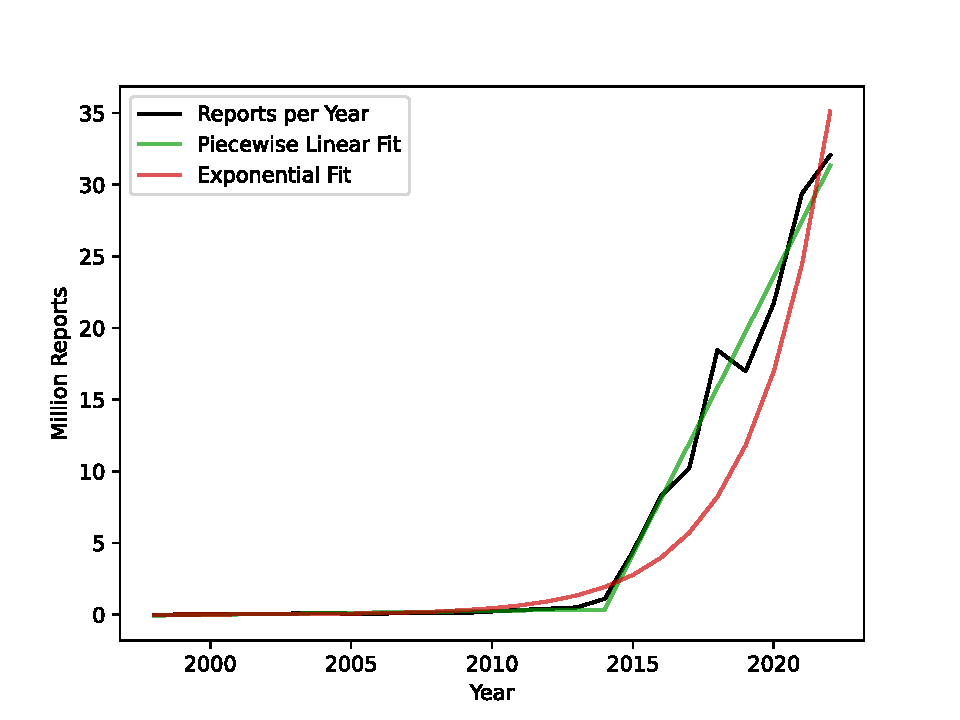
\includegraphics[
    scale=0.6,
    alt={A line chart plotting the growth of yearly CyberTipline reports from
    1999 through 2022. While described as exponential by NCMEC, a piecewise
    linear least-squares fit comes closer, with growth sharply accelerating
    after 2014 to double every four years.}
]{figure-reports-per-year}
\caption{Yearly CyberTipline reports (per NCMEC)}
\Description{A line chart plotting the growth of yearly CyberTipline reports
from 1999 through 2022. While described as exponential by NCMEC, a piecewise
linear least-squares fit comes closer, with growth sharply accelerating after
2014 to double every four years.}
\label{fig:yearly-reports}
\end{figure}

Figure~\ref{fig:yearly-reports} plots yearly reports since inception of the
CyberTipline in February 1999 as a black line. It also shows two
least-squares-fit lines, with the piece-wise linear fit in green and the
exponential fit in red. In its \V{OJJDP} report, \V{NCMEC} describes this growth
as ``exponential.'' While the sharp acceleration around 2014 does remind of
exponential curves, the growth before 2014 and after 2014 didn't consistently
accelerate. In fact, growth has been slowing of late and, given Meta's markedly
smaller piece counts for the first three quarters of 2023 as shown in
Figure~\ref{fig:meta-pieces}, its average pieces to reports ratio as discussed
in Section~\ref{sec:pieces-and-reports} below, and its over 80\% share of all
CyberTipline reports, that slowdown will very likely hold for 2023 as well.

\begin{table}
\centering\libertineLF
\caption{CyberTipline violative activities in descending order for 2022 (\V{NCMEC})}
\label{tab:report-contents}
\begin{tabular}{l|rr|rr|rr}
\textbf{Activity}
& \textbf{2020} & \textbf{\%}
& \textbf{2021} & \textbf{\%}
& \textbf{2022} & \textbf{\%}
\\ \hline
Child pornography & 21,669,264 & 99.62383 & 29,309,106 & 99.69870 & 31,901,234 & 99.50780 \\
Online enticement for sexual acts & 37,872 & 0.17412 & 44,155 & 0.15020 & 80,524 & 0.25117 \\
Obscene material sent to child & 3,547 & 0.01631 & 5,177 & 0.01761 & 35,624 & 0.11112 \\
Child sex trafficking & 15,879 & 0.07300 & 16,032 & 0.05453 & 18,336 & 0.05719 \\
Child sexual molestation & 11,770 & 0.05411 & 12,458 & 0.04238 & 12,906 & 0.04026 \\
Misleading words/images online & 8,689 & 0.03995 & 5,825 & 0.01981 & 7,517 & 0.02345 \\
Misleading domain name & 3,109 & 0.01429 & 3,304 & 0.01124 & 1,948 & 0.00608 \\
Child sex tourism & 955 & 0.00439 & 1,624 & 0.00552 & 940 & 0.00293 \\
\end{tabular}
\end{table}

Table~\ref{tab:report-contents} breaks down CyberTipline reports by violative
activity from 2020 to 2022. Rows are sorted in descending order of counts for
2022. As the table makes ample clear, the vast majority of reports, over 99.5\%,
concerns child pornography or \V{CSAM}. At the same time, the remaining fraction
of a percent of reports still represents devastating harm to minors. For
example, \V{NCMEC} separately discloses that in 2022 1.66~reports have the same
perceptually similar attachments and hence are redundant. If we assume a similar
relationship between reports and victims for sex trafficking, 18,336 reports for
that activity in 2022 correspond to more than 11,000 minors being trafficked,
which is an uncomfortably large number even in a global context.


\subsection{CyberTipline Reports and Their Attachments, i.e., Pieces}
\label{sec:pieces-and-reports}

\begin{table}
\centering\libertineLF
\caption{CyberTipline reports and attached pieces (\V{NCMEC})}
\label{tab:reports-pieces}
\begin{tabular}{l|rr|r|rr|rr}
\textbf{Year} & \textbf{Reports} & $\pi$ & \textbf{Pieces}
& $\pi$ & \textbf{Unique Pieces} & $\pi$ & \textbf{Similar Pieces} \\ \hline
2020 & 21,751,085 & 3.00 & 65,344,724 & 2.39 & 27,333,171 & 4.62 & 14,141,118 \\
2021 & 29,397,681 & 2.88 & 84,795,507 & 2.32 & 36,625,281 & 3.85 & 22,005,389 \\
2022 & 32,059,029 & 2.72 & 87,179,813 & 2.01 & 43,399,901 & 3.21 & 27,136,862 \\
\end{tabular}
\end{table}

Table~\ref{tab:reports-pieces} relates CyberTipline reports and attached pieces,
that is, pictures, videos, and other documents (including \V{PDF} files). It
provides a global view in addition to the platform-specific data already
included in Table~\ref{tab:meta-pieces-and-reports} for Facebook and Instagram,
Table~\ref{tab:alphabet} for Google and YouTube, Table~\ref{tab:pinterest} for
Pinterest, Table~\ref{tab:reddit} for Reddit, and Table~\ref{tab:snap} for Snap.
Columns labelled $\pi$ for \emph{product} show the multiplicative factor
relating grouped counts to the number of pieces in the fourth column. Unlike
previous tables, Table~\ref{tab:reports-pieces} counts pieces in three different
ways:
\begin{itemize}
    \item Column \#4 contains the total number of pieces (as in other tables).
    \item Column \#6 contains the number of unique pieces, filtered with \V{MD5}.
    \item Column \#8 contains the number of perceptually similar pieces,
    filtered with PhotoDNA and Videntifier.
\end{itemize}
In other words, the sixth column doesn't count a photo or video if the \V{MD5}
hash function produces the same value as for a previously counted photo or
video. Likewise, the eighth column doesn't count a photo or video if the
PhotoDNA or Videntifier perceptual hash function produces a similar value. The
critical difference between the two kinds of hash functions is that a small
change in input to \V{MD5} produces a completely different value, whereas a
small change in input to PhotoDNA or Videntifier produces almost the same value,
thus allowing for the detection of visually similar material~\cite{Farid2021}.
Alas, the use of \V{MD5}, PhotoDNA, and Videntifier also is highly problematic.

First, cryptographically secure hash functions should make it practically
impossible to construct an input for a given output. While that isn't practical
for \V{MD5} in the most general case, so-called preimage attacks, it \emph{is}
practical for more restricted cases, notably chosen prefix
attacks~\cite{StevensLenstraea2012}. But even a single known pair of colliding
inputs, which have been published for \V{MD5} and \V{SHA1}, suffices for
constructing pairs of \V{PDF} documents with different visible contents and
identical hashes~\cite{LeurentPeyrin2020,StevensBurszteinea2017}. With some
limitations, images in the \V{JPG} and \V{PNG} formats as well as videos in the
\V{MP4} format are vulnerable to such attacks as
well.\footnote{\url{https://github.com/corkami/collisions}}

If internet platforms and \V{NCMEC} use \V{MD5} hashes to identify \V{CSAM}
without human intervention, as they apparently do already, that opens up the
possibility of attacks that are designed to close down accounts or to trigger a
law enforcement investigation akin to swatting. An attacker would need access to
at least one known \V{CSAM} hash, construct a document that has the same hash,
and socially engineer the targeted user into posting that document. Given the
devastating consequences of a false positive for \V{CSAM}~\cite{Hill2022}, the
possibility of such attacks argues strongly against the continued use of
\V{MD5}---and \V{SHA1} for that matter. However, even though these
vulnerabilities aren't particularly new, dating back to 2012 and 2017, \V{NCMEC}
was still asserting in 2023 that ``[i]mages that share the same \V{MD5} hash are
identical,'' displaying no awareness of the problem~\cite{NCMEC2024}.

Second, Microsoft's PhotoDNA~\cite{Farid2018} is widely used for \V{CSAM}
detection, probably as a result of the firm making the technology freely
available to organizations such as \V{NCMEC}. While Microsoft has kept the exact
algorithm secret, it has not only been reverse-engineered~\cite{Krawetz2021a},
but practical second preimage attacks have been
documented~\cite{ProkosJoisea2021}. Furthermore, despite Microsoft's claims
otherwise, it may be possible to recreate low resolution versions of the
original images from PhotoDNA hashes, i.e., \V{CSAM}~\cite{Athalye2021}. In
other words, PhotoDNA is even more susceptible to adversarial abuse than
\V{MD5}~\cite{Steinebach2023}.

Third, little is known about Videntifier's algorithm, which was developed by the
eponymous Icelandic firm in collaboration with \V{NCMEC}. That makes it
impossible to assess its strengths and weaknesses. While PhotoDNA's history
suggests that such secrecy can delay but not prevent public scrutiny, the more
troubling lesson from other perceptual hash algorithms is that they just aren't
very robust. Notably, Meta's \V{PDQ}~\cite{DavisRosen2019} doesn't perform all
that well and is also vulnerable to second preimage
attacks~\cite{Krawetz2022,ProkosJoisea2021}. Despite relying on a machine
learning model to identify image features, Apple's NeuralHash suffers from
similar limitations, including (again) susceptibility to second preimage
attacks~\cite{StruppekHintersdorfea2022}.

When comparing overall and platform-specific report and piece counts, Meta's and
Snap's numbers are fairly close to the overall ratio. But Google's and YouTube's
are significantly larger, whereas Pinterest's and Reddit's are significantly
smaller. Since Google, Reddit, and YouTube passed audits of their report counts
and Pinterest's report counts aren't that far off, these discrepancies most
likely reflect real differences in platform usage and content moderation.
However, only the platforms are in a position to identify what factors make the
difference and none of them provide an explanation. Such divergences between
platform-specific and industry-wide statistics are not covered in any best
practices guidelines but also are just the phenomena that stick out when closely
examining transparency disclosures.


\subsection{Global Distribution of CyberTipline Reports}
\label{sec:spread}

To consider the global spread of \V{CSAM}, I turn to \V{NCMEC}'s reports per
country covering 2019--2022~\cite{NcmecByCountry2019,NcmecByCountry2020,
NcmecByCountry2021,NcmecByCountry2020}. As discussed above, the data does have
minor quality issues, but they impact less than 0.001\% of the reports, i.e.,
are negligible. However, making meaningful comparisons between countries also
requires normalizing the data. While the number of countries' internet users
would form the most suitable denominator, I could not find an up-to-date and
accurate dataset with that information. Almost all datasets claiming to do so,
including the Worldbank's, trace back to the International Telecommunication
Union (\V{ITU}). But that dataset has not been updated for years for many
countries and provides percentage fractions of countries' populations only.
Instead of scaling population counts by outdated and hence unreliable fractions,
I instead decided to use population counts by themselves. In particular, the
United Nations provide up-to-date, yearly statistics, even if they often are
(informed) estimates.

That normalization strategy also is the first of two major caveats about my use
of reports per capita, country, and year in this section. If different countries
have significantly different shares of internet users when compared to the
entire population, then their reports per capita, country, and year will be
skewed proportionally and hence their absolute magnitudes are incomparable.
Though relative trends will still be meaningful. In practice, comparisons based
on reports per capita favor Sub-Saharan African countries, which have much lower
internet penetration than much of the rest of the world. That is reflected in
the data: When ranking all subcontinental regions by absolute CyberTipline
report counts, West-, East-, and Southern Africa place in the third quartile.
But when ranking them by reports per capita, the three regions place in the
fourth quartile.

Independent of dataset used for normalization, it's a good idea to drop
localities with tiny populations. For instance, in 2021, the Cocos (Keeling)
Islands, an Australian territory in the Indian Ocean south-westish of Sumatra,
had a population of 593 and 168 CyberTipline reports. The resulting outlier of
0.283 reports per capita is seven times larger than the next largest quantity of
0.040 over all four years. On a linear, continuous color scale (which nicely
avoids futzing with histogram binning strategy, one of the dark arts of data
visualization), that effectively compresses the color range for all other
countries to shades surprisingly similar to that for zero.

The second major caveat concerns the numerator, i.e., report counts. If
countries' online populations significantly differ in what platforms they use,
then cumulative report counts may be more reflective of differences in \V{CSAM}
detection than differences in populations' \V{CSAM} usage. That is trivially the
case for countries with a large share of platforms that are not \V{US}-based,
notably the People's Republic of China. While the country appears in \V{NCMEC}'s
disclosures, with a maximum of 7,644 reports for 2021, the small number most
certainly is a direct result of China banning many foreign websites and services
including social media. In fact, out of the 16 surveyed platforms and firms,
only Microsoft Bing and Skype, Snap, and Wordpress were accessible through
Top10VPN's testing
tool\footnote{\url{https://www.top10vpn.com/tools/blocked-in-china/}} in January
2024. North Korea's international rogue status is similarly reflected in the
data: Its maximum was 9 reports in 2020. By comparison, South Korea, with about
double the population, had 100,709 reports that same year.

I believe that a comparison based on reports per capita, country, and year still
is meaningful thanks to Meta's astounding global reach and its overwhelming lead
in reporting \V{CSAM}. Notably, over the four years covered by \V{NCMEC}'s
disclosures, the size of Meta's family monthly active people grew from 2.69
billion during \V{Q1}~2019 to 3.74 billion during \V{Q4}~2022. That is 35--47\%
of the world population including China---or 43--57\% excluding China! Meta also
was responsible for 94.3\% of all \V{CSAM} reports in 2019, 94.7\% in 2020,
92.2\% in 2021, and 85.5\% in 2022. In other words, the vast majority of
CyberTipline reports reflect Meta's screening for \V{CSAM} amongst the roughly
half of humanity counting as the firm's monthly users.

\begin{figure}
\centering
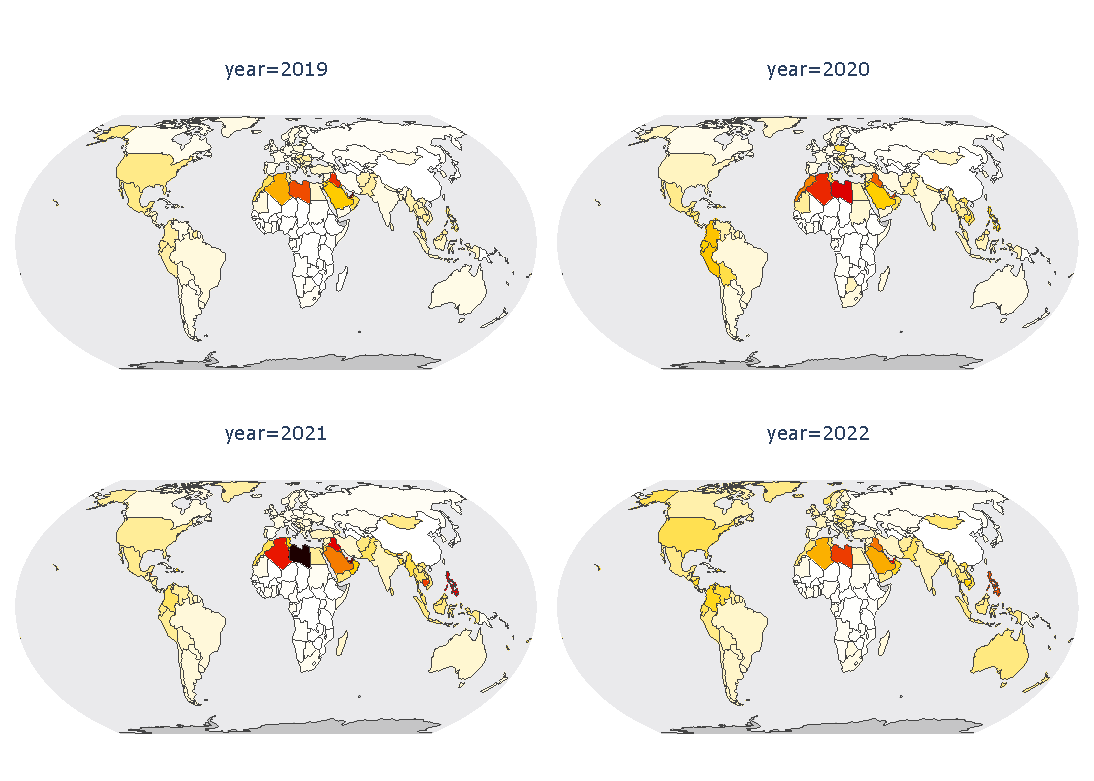
\includegraphics[
    scale=0.8,
    alt={Figure with four choropleths plotting the CyberTipline reports per
    capita, country, and year for 2019 through 2022. North African and Middle
    Eastern countries are shaded in dark colors in all four panels, representing
    consistently very high reports per capita for most Arab League countries,
    whereas most other countries become successively darker over the four years due
    to a doubling of total reports over that period.}
]{figure-reports-per-capita}

\caption{Reports per capita, country, and year. The four choropleth panels plot
CyberTipline reports per country and year over \V{UN} population size per country
and year using an Equal Earth projection. Colors continuously range between
white for 0.000 through yellow and red to black for 0.040.}
\Description{Figure with four choropleths plotting the CyberTipline reports per
capita, country, and year for 2019 through 2022. North African and Middle
Eastern countries are shaded in dark colors in all four panels, representing
consistently very high reports per capita for most Arab League countries,
whereas most other countries become successively darker over the four years due
to a doubling of total reports over that period.}
\label{fig:reports-per-capita}
\end{figure}

Figure~\ref{fig:reports-per-capita} illustrates reports per capita, country, and
year, using \V{UN} population data to normalize report counts, a colorscale
capped by the maximum value over all four years, and the Equal Earth
projection~\cite{SavricPattersonea2019}. In addition to being aesthetically
pleasing, that projection is equal-area and hence suitable for choropleths. Maps
for 2019 and 2020 are largely consistent with the map included in
in~\cite{BurszteinBrightea2019} based on earlier, non-public \V{NCMEC} data.
Assuming that their analysis is subject to similar limitations as mine, which is
reasonable given that they too start with CyberTipline report counts, the
consistency suggests that \V{CSAM} sharing patterns did not much change between
the two studies.

Alas, my analysis does surface one oddity: Members of the 22-country strong Arab
League have noticeably high reports per capita over the covered four years;
though they markedly and consistently decline over that time span as well. At
the extreme, either the United Arab Emirates or Libya is the country with the
most reports per capita for each of the four years. Meanwhile the decline
becomes obvious if we treat the Arab League as a country: It would rank 15th,
18th, 19th, and 26th, respectively. Furthermore, per capita rates for those
countries do not increase whereas those for the rest of the world do increase,
with the total number of reports doubling from 2019 to 2022. While I cannot
explain this oddity, the fact that the United Arab Emirates and Libya are
highest ranked for two out of four years even though they are polar opposites
when its comes to wealth and political stability does point to some shared
cultural trait. Alas, that shared trait may very well be a bias by content
moderation systems!


\subsection{Relationship between Victims and Offenders}

In addition to providing additional data on CyberTipline reports, \V{NCMEC}'s
report to the Office of Juvenile Justice and Delinquency
Prevention~\cite{NCMEC2023} also contains information about its Child Victim
Identification Program, which maintains a separate database tracking the
identities of minors appearing in \V{CSAM}. Apparently, many law enforcement
agencies contribute \V{CSAM} found during investigations to the database and
also provide, if known, information about the relationship between victims and
suspected offenders. Unfortunately, \V{NCMEC} presents this information broken
down by pieces and unique pieces but not by person. Furthermore, while yearly
piece counts are just below or well over one million, the number of minors in
the database appears to be much smaller. In particular, \V{NCMEC} added 773
minors in 2020, 1,477 minors in 2021, and 4,464 minors in 2022. Given the small
number of victims, I also report equivalent statistics published by \V{OJJDP}
based on the \V{FBI}'s National Incident Reporting System Master Files for 2018
and 2019~\cite{OJJDPStats2022}.

The majority of suspects are members of the victim's extended family, accounting
for 64.2\% of all unique pieces in 2022. That includes fathers with 30.4\%,
step-fathers with 8.1\%, uncles with 8.0\%, and the guardian's partner with
6.3\%. Another 24.6\% are socially familiar, including family friends,
neighbors, and teachers. The rest are online enticement with 9.3\%, trafficking
with 1.4\%, and strangers with 0.5\%. By comparison, \V{OJJDP}'s statistics
attribute 53.1\% to a victim's family, 44.7\% to acquaintances, and 2.2\% to
strangers. If we treat online enticement as involving acquaintances as well, the
statistics are roughly the same, with the offenders being family members in the
clear majority of cases and strangers in less than one thirty-second.

It seems safe to conclude that drag queens, which count as strangers, do not
figure prominently as threats. However, fathers and step-fathers most certainly
do. Hence, moms for liberation would be well advised to reject the yoke of
child-abusing patriarchy and instead rear their children within lesbian
relationships!


\subsection{Missing Data on Teenage Sexting}

\V{NCMEC} provides statistics on age and gender only for minors newly added to
its Child Victim Identification Program but not for CyberTipline reports. But
even if it did, that wouldn't suffice for separating out reports about voluntary
and consensual teenage sexting. I am highlighting sexting because it is very
popular, with prevalences in a recent meta-analysis at 19.3\% for sending,
34.8\% for receiving, and 14.5\% for forwarding without
consent~\cite{MoriParkea2022}. While the latter is ethically problematic, the
harsh penalties of Chapter~110 hardly seem an appropriate tool to foster teenage
learning. Yet according to federal law, teenage sexting qualifies as \V{CSAM}
all the same.

Advocating an abstinence-only approach to sexting is bound to fail just like
prior abstinence-only sex education did, despite the \V{US} spending over \$2
billion on such programs since the 1990s~\cite{FoxHimmelsteinea2019}. While
\V{NCMEC} doesn't quite advocate abstinence, its webpage on the
topic\footnote{\url{https://www.missingkids.org/netsmartz/topics/sexting}.}
seems rather dismissive of teenagers who are sexting, featuring the above
statistics under the technically correct but nonetheless misleading heading
``Most Teens Are Not Texting,'' and then offers only potential negative
consequences under ``Protect yourself,'' none of them actionable advice that
might help teenagers protect themselves. Furthermore, the page does recommend
reporting any inappropriate incident to the CyberTipline, reassuring readers
that ``it is not the child who is at fault.'' Given \V{US} law, that seems
positively misleading.

While federal prosecution of sexting teenagers is unlikely, the same cannot be
said for \V{US} states. 23~out of 50~states have no exemption for consensual
sexting by teenagers on the books. The other 27~do, but still punish even
consensual sexting, typically as a misdemeanor~\cite{HindujaPatchin2022,
HoloydaLandessea2018,StrasburgerZimmermanea2019}. Worse, lower penalties may
have the pervese effect of making state prosecutors \emph{less} reluctant to
charge teenagers~\cite{Hasinoff2016}. Even if that isn't the case, 62\% of state
prosecutors in one survey have handled such cases and 36\% initiated
prosecutions~\cite{WalshWolakea2013}. While they claim to have done so largely
for cases where teenagers were abusive, it takes little effort to find examples
where that was not the case, often with disastrous consequences including
suicide~\cite{Dunlap2016,Feldman2020,Jouvenal2023,LorangMcNielea2016,Miller2015,
WolakFinkelhorea2012}. Against that background, \V{NCMEC}'s apparent
indifference to the topic and the lack of data on its share amongst CyberTipline
reports is positively troubling.


\subsection{Summary}

Overall, the analysis of available transparency data on the sexual exploitation
of minors shows an alarming growth of detected imagery and other activities over
the last decade and hence is in line with similar observations by, say, the New
York Times~\cite{Dance2019,KellerDance2019}. In particular, since the vast
majority of that growth is due to a single organization, Meta, much of that
growth is very likely true growth and not attributable to improved awareness and
detection technology. The analysis also suggests that existing detection
technology, notably \V{\V{MD5}} and PhotoDNA, is easily abused and hence should
be phased out. At the same time, Meta's investigation of apparent intent and the
lack of data on teenage sexting also suggest that current statistics are not
sufficiently differentiated and hence significant overcounts. Clearly, more
robust detection technology and more fine-grained statistics are urgently
needed!


% ======================================================================================

\section{Discussion}
\label{sec:discussion}

Since audits and analysis have different overall thrusts, distinguishing between
them for structuring this paper's exposition made eminent sense. But in
practice, the distinction between audits and analysis was far less clear and
their connection more organic: I simply kept poking at the data to make sense of
available statistics. In my mind, the transition from just poking quantities to
telling a coherent story grounded in the data is just what needs to happen for
transparency disclosures to result in meaningful accountability. That suggests
several takeaways about transparency disclosures in general and about their
presentation. I start with higher-level observations.

First and not surprisingly, there is a bottom threshold for metrics and data to
be useable in data-driven story telling. In particular, without having overall
statistics on the relationship between CyberTipline reports and pieces, the
varying platform-specific ratios were impossible to classify. \V{NCMEC}'s
publication of its report to the Office of Juvenile Justice and Delinquency
Prevention (\V{OJJDP}) not only filled that hole but provided several more
helpful statistics.

Second and more unexpectedly, there is value even in incomplete or buggy
transparency disclosures \emph{as long as} they can be combined with similar
disclosures by other organizations. It helps when one organization's disclosures
are general and robust enough to provide a foundation, as \V{NCMEC}'s \V{OJJDP}
report did for the previous section. But with that backbone in place, I could
rely on platform-specific disclosures to add interesting detail, even if they,
like Pinterest's, were not entirely accurate. That should serve as warning
against simply dismissing existing disclosures as ``transparency
theater''~\cite{Douek2022}.

Third, transparency disclosures run counter the scientific method. Quite
literally: The latter requires the formulation of hypothesis and research
questions before the selection of metrics and, if not already available, the
collection of data. Yet here, civil society and other interested outsiders need
to make do with the data already collected and disclosed by platforms. While
actual practice isn't quite as lopsided as that (with civil society influencing
platforms' practices to some degree), this \emph{modus operandi} is reflective
of data ``science'' in general and leads to predictably imprecise results. To
stick to theatrical metaphors: If you were performing to an empty room every
night, how much effort would you put into your performance?

The implication is that meaningful platform transparency requires
\emph{continuous} engagement with outside stakeholders. It also requires
adjusting disclosed metrics in response to outside questions, e.g., about
teenage sexting. That does complicate life for regulators, who would prefer to
just pick from a menu of internationally agreed upon
metrics~\cite{HarlingHenesyea2023}. However, keeping disclosure requirements
adaptable does not mean that regulation is inadvisable or
impossible~\cite{Douek2022,Klonick2023}. On the contrary, as I argued above,
Meta sticking with its historical disclosures after two years of significant
churn illustrates the beneficial impact of regulation. Similarly, the \V{EU}'s
statements of reasons database promises to enable more scrappy audits for all of
content moderation~\cite{TrujilloFagniea2024}. At the same time, an effective
regulator really needs to have their own research and data divisions to engage
platforms~\cite{Jaursch2022a,Jaursch2023}.

In addition to these more general observations, I do have concrete suggestions
for improving transparency disclosures. Notably, fancy, irregular layouts and
statistics embedded in text obfuscate the data. \V{NCMEC} actually did start
reporting violative activities and attached pieces a year earlier, in its
CyberTipline 2021 Report~\cite{NcmecCyberTipline2021}. But that didn't register
when I scanned the written report because of the layout and long passages of
low-information text. Meanwhile, the more focused presentation of the \V{OJJDP}
report with its simple, inline tables registered immediately.

Having said that, raw counts in machine-readable form, i.e., \V{CSV}, are
\emph{much preferrable}. Having to say so for data originating from some of the
largest technology firms in the world feels a bit surreal. But the fact that
many of them fail to do so even for \V{DSA} disclosures despite the act's
explicit requirement only underlines the importance of this point. Also, do not
round numbers. They are inaccurate and (literally) do not add up. Do not include
(percentage) fractions. They almost always are rounded as well and hence
inaccurate. Worse, if the original denominator isn't readily available, they get
in the way of recovering counts. That is the case for TikTok's \V{CSE}
disclosures as well as for the \V{ITU}'s data on internet users per country.


\section{Outlook}
\label{sec:outlook}

To improve the accountability of social media platforms, I audited the
transparency disclosures of 16 major platforms by comparing redundantly or
repeatedly disclosed quantities. Even though the audit methodology is rather
basic and I focused on an area with clear legal reporting mandates, the sexual
exploitation of minors, audit results were not exactly encouraging. Out of the
16 surveyed platforms operated by 11 technology firms:
\begin{itemize}
\item[\ding{56}] 3 platforms do not make transparency disclosures;
\item[\ding{56}] 2 platforms do not make transparency disclosures about content moderation;
\item[\ding{56}] 3 platforms make such disclosures but do not meet audit requirements;
\item[\ding{56}] 3 platforms failed the audit of repeatedly disclosed historical data;
\item[\ding{56}] 1 platform failed the audit of redundantly disclosed CyberTipline reports;
\item[\ding{52}] 4 platforms passed the audit of redundantly disclosed CyberTipline reports.
\end{itemize}
Despite these significant shortcomings, the existing data still helps
characterize the sexual exploitation of minors across social media platforms and
countries. At the same time, the overview would have been impossible without
more comprehensive disclosures by the clearing house for reporting such
activities, \V{NCMEC}.

Based on my experiences with audits and analysis, I argued that meaningful
transparency disclosures require continuous engagement by platforms and civil
society alike. But getting social media firms to fully embrace such an iterative
transparency process and make good faith disclosures may turn out to be
difficult. Meta illustrates why. The firm has been industry-leading in its
efforts to suppress the spread of \V{CSAM}. Not only does it detect the vast
majority of cases, but it has the longest track record of releasing statistics
to the public, has consistently supported \V{NCMEC} over the last several years,
with two employees serving as board members until recently, and performed
helpful research to better characterize the sheer volume of \V{CSAM}.

But as my audit demonstrated, those transparency disclosures also suffer from
serious data quality issues. Meta similarly misreported advertising metrics to
customers~\cite{BruellPatel2020,Hutchinson2016,Hutchinson2016b,Hutchinson2017,
VranicaMarshall2016}, platform usage data to a Harvard-based research
consortium~\cite{Timberg2021}, and adverts in its transparency
database~\cite{Rosenberg2019,ScottMontellaro2021,SilvermanMac2020a}. Human error
is a plausible explanation in all these cases. Though one research group with
consortium access to Meta's data also published a rather pointed critique about
its quality well before the discovery that the dataset was incomplete and hence
unusable~\cite{Hegelich2020,HegelichMarcoea2020}. That experience prompted even
the consortium head to call for industry-wide
regulation~\cite{PersilyTucker2021}.

Meanwhile, moving too fast does not suffice for explaining several other cases.
Notably, Meta kept violating non-discrimination laws in advertising for years,
despite having been repeatedly notified of its
noncompliance~\cite{AngwinParrisJr2016,AngwinScheiberea2017,AngwinTobinea2017,
KofmanTobin2019,Kofman2022,Merrill2020,TobinMerrill2018}. Next, as I discovered
during my employment, the firm also manipulated view impressions, only the most
basic advertising metric, to its own economic benefit~\cite{Grimm2022c}. Despite
its significant efforts on minor safety, the firm did run an advertising
campaign (for TikTok nonetheless) that sexualized teenage girls for the benefit
of middle-aged straight men. When employees raised concerns, the firm cut off
their access to information about the ad campaign but otherwise continued
running the ads~\cite{SilvermanMac2020}. In the aftermath of the \V{US}
presidential election and attempted coup and facing a barrage of criticism, Meta
deplatformed the academics who had been collecting the data enabling many of the
above news reports about the firm's ad database~\cite{EdelsonMcCoy2021,
EdelsonMcCoy2021a}. At that time, the firm also disbanded the team responsible
for its CrowdTangle transparency tool~\cite{Roose2021a}, with the project's
founder leaving the firm a few months later~\cite{Heath2021} and Meta
``pausing'' sign-ups for new users a few more months
later~\cite{PatelCulliford2022}.

With the Digital Services Act, the \V{EU} created a powerful but measured,
multipronged oversight and enforcement mechanism. On paper, the \V{DSA} more
than suffices for reigning in a firm with a long track record of moving either
too fast or too deviously. However, doing so in practice will likely require
active intervention to prod Meta into compliance. Whether the commission and
member countries' regulators can muster the necessary stamina and wherewithal is
an open question. Unfortunately, their track record over six years with \V{GDPR}
is less than impressive~\cite{Burgess2022}. In other words, we are well-advised
to grow the arsenal of scrappy audits and other means for holding social media
accountable. Luckily, the \V{EU} Commission has already provided us with a new
tool for doing so through the statements of reasons database. While other
researchers have already performed a first comparison of database entries with
aggregate \V{DSA} transparency disclosures, I am particularly interested in
fully automating these audits to hold social media accountable for correct
counts when it comes to transparency!


% ======================================================================================

\begin{acks}
An \V{NCMEC} employee helped complicated my thinking about \V{CSAM}---while
somehow also avoiding to answer any of my questions. Meanwhile Karin Wolman did
answer my questions about 18 \V{US} Code. Thank you both!
\end{acks}

\bibliographystyle{ACM-Reference-Format}
\bibliography{bibliography}

\end{document}
